\documentclass[main.tex]{subfiles}

% The following commands are from the \textpages macro
% and are needed for the subfile properly.
% These commands are ignored when compiling main.tex
\pagestyle{empty}
\cleardoublepage
\pagestyle{myheadings}\markboth{}{}
\def\@chapapp{\protect\@textofChapter}
\def\Thechapter{\arabic{chapter}}
\pagenumbering{arabic}
% End of commands


\begin{document}

\chapter{Some content}

% The following block creates a box for citing your publications in the chapter.
% You can begin to write the chapter text from the marker below.
% Delete this box if desired.
\begin{tcolorbox}[float=b,
                  width=\textwidth,
                  %boxsep=0pt,
                  left=1em,
                  right=1em,
                  top=0.5em,
                  bottom=0.5em,
                  %colback=white,
                  boxrule=0pt,
                  colframe=white,
                  %sharp corners
                  ]%%
    \footnotesize
    \uwsinglespace
    Parts of this chapter were published as:
    
    \vspace{0.5em}
    % Modify the citations below here, tabular environment is to enable multiple citations and hanging indentation.
    % Add the citations in the bibliography here to cross reference.
    % You must manually enter the information but you can choose the format
    \begin{tabularx}{1\textwidth}{l X}
        \cite{} & F. M. Last, U. R. Advisor, ``Article 1 title,'' \textit{Journal name} \textbf{1}, pp.~123 (2025). \\
        \cite{} & F. M. Last, U. R. Advisor, ``Article 2 title,'' \textit{Journal name} \textbf{2}, pp.~456 (2025).
    \end{tabularx}
\end{tcolorbox}

% --------------------------------
% Add chapter main text below here
% --------------------------------


\section{First section}
Lorem ipsum dolor sit amet, consectetur adipiscing elit. Fusce volutpat euismod mi sit amet consectetur. Fusce ut convallis mi, quis facilisis mi. Donec rhoncus rutrum tellus a iaculis. Quisque sit amet neque neque. Proin cursus ipsum mi, sed interdum diam condimentum non. Proin vulputate nisl id vehicula gravida. Nulla facilisi. Proin euismod aliquam dolor sed aliquet. Nullam eu libero purus. Donec lacinia cursus est. Fusce ante mauris, pretium eget lacinia vel, vestibulum sit amet urna. Proin et arcu suscipit, volutpat magna a, ornare leo. Suspendisse pharetra sapien dui, cursus elementum eros euismod a. Mauris turpis odio, tincidunt ut pellentesque id, efficitur ut elit. Suspendisse elit leo, varius et mauris sed, consectetur rutrum enim. Nam ullamcorper semper ipsum, nec tristique ex gravida nec.

Duis scelerisque libero sed ipsum rutrum, eget egestas ante aliquam. Nunc dictum suscipit felis id placerat. Duis sagittis augue eget justo ultricies posuere. Maecenas eu urna sed enim maximus auctor. Ut sit amet sem dolor. Aenean tempor purus ac rhoncus posuere. Quisque rhoncus ligula odio, id tincidunt diam egestas quis. Vestibulum quis massa non ligula hendrerit laoreet. Proin at erat imperdiet, vehicula augue consectetur, convallis erat. Cras porta laoreet arcu, porttitor vehicula nisl luctus vel. Morbi pulvinar sollicitudin diam ac rhoncus. Aenean et scelerisque nisi. Proin et nulla mi.

Phasellus imperdiet condimentum lectus a laoreet. Quisque hendrerit mi at urna egestas venenatis. Etiam aliquam purus lobortis lorem interdum ornare. Etiam commodo nunc non finibus varius. Nulla tempus, magna vel mattis laoreet, ex enim convallis neque, vel hendrerit tellus elit sed ligula. Duis augue elit, malesuada sed aliquam et, commodo sed ante. In magna felis, pulvinar tristique nulla sed, ultrices euismod turpis. Fusce quis justo purus. Quisque tristique purus felis, at posuere augue aliquet aliquet. Fusce sagittis malesuada orci, quis facilisis justo vehicula a. In erat augue, consectetur id sagittis non, vulputate at arcu.

\begin{figure}[t]
    \centering
    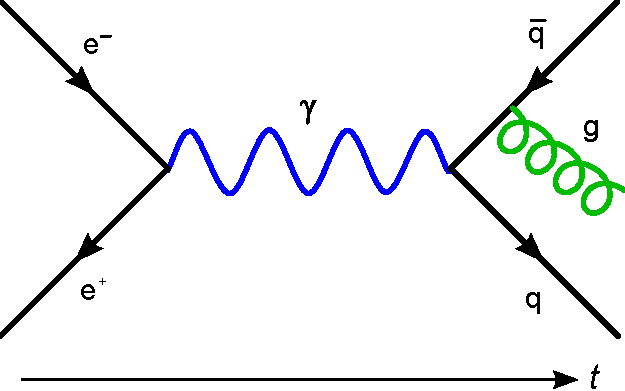
\includegraphics[width=0.5\textwidth]{figures/ch2/sample.pdf}
    \caption{
        Figure caption. Another change relative to the main style file is that the figure captions are single spaced. You can go into the style file to adjust this if desired.
    }
    \label{fig:ch2:sample}
\end{figure}

Sed at metus ut ex sagittis ultrices vitae ut odio. Pellentesque vitae molestie ipsum. Praesent fringilla magna vel erat auctor, id congue risus sodales. Vestibulum ut egestas ipsum. Duis cursus nunc ut rutrum tristique. Nullam vulputate erat diam, eget vulputate odio dictum quis. Aenean scelerisque felis semper diam pharetra pellentesque et et nulla. Sed varius ullamcorper quam, non sodales magna pharetra ac. Nunc ut felis vitae tellus malesuada finibus.


\end{document}